\documentclass[output=paper]{langsci/langscibook} 
\title{Intonation and emotions in Kɔnni: A preliminary study} 
\author{%
 Michael Cahill\affiliation{SIL International} 
}
% \sectionDOI{} %will be filled in at production

\abstract{ 
One of the paralinguistic functions of intonation is the use of gradient changes of pitch and duration to indicate emotional states of the speaker. This study examines the difference in pitch of Kɔnni native speakers' speech which accompanies several different emotions. A neutral utterance was compared to the same sentence uttered as if the speakers were surprised, bored, angry, ``contemptuous", and wanted to emphasize the sentence. Base pitch level, pitch range and overall duration of the sentences were measured and compared to the neutral statement. The results of this study are compatible with those found in other languages, and add to the knowledge of how tone languages are able to express paralinguistic intonation in a systematic way.
}

\maketitle
\begin{document}



\section{Introduction}
The term \emph{intonation} does not have a universally agreed on definition. Some researchers either explicitly define it in terms of pitch alone or seem to assume such a definition (\citealt{lieberman1967}; most papers in \citealt{bolinger1972,gussenhoven2004}). As \citet[3]{hirstdicristo1998} note, the terms \emph{intonation} and \emph{prosody} have often been used interchangeably in the literature. These authors spend significant time discussing the ambiguities of various terms, distinguishing \emph{intonation proper}, which deals with pitch, from the broader term \emph{prosody}, which also includes intensity and quantity. \citet[4]{ladd2008} gives a useful definition which we will assume here: ``the use of \emph{suprasegmental} phonetic features to convey 'postlexical' or \emph{sentence-level} pragmatic meanings in a \emph{linguistically structured} way'' (his emphasis). Though pitch will be the most common measure referred to in this paper, duration will also be examined. 

A particular instance of intonation can be either \emph{structural} or \emph{paralinguistic} (\citealt{gussenhoven2004,laddetal1986,ladd2008}). \emph{Structural} intonation is categorical and phonological, indicating linguistic boundaries or morphosyntactic functions. \emph{Paralinguistic} intonation involves gradient phonetic values of pitch, as well as duration and intensity, often indicating emotions and attitudes. Kɔnni has cases of each of these, and a broader range of intonational patterns is examined in \citet{cahillforth}, but this paper's focus will be on paralinguistic intonation.

Intonation in tone languages has not been studied nearly as much as in non-tonal languages, probably on the assumption that lexical and grammatical tone would override any pitch differences attributable to intonation.\footnote{An exception to this will be a volume entirely devoted to intonation in African languages, edited by Laura Downing and Annie Rialland (De Gruyter, \citeyear{downingriallandforth}). This will include my broader review of several intonation patterns in Kɔnni.} The papers on various languages in \citeauthor{hirstdicristo1998}'s (1998) survey include a few tone languages (Thai, Vietnamese, and Beijing Mandarin), and the papers on Thai and Vietnamese have some detailed remarks on the topic of this paper: how emotional states influence intonation. However, the overall literature on emotions and intonation in tone languages is still sparse. \citeauthor{green2009}'s (2009) work titled ``Prosody and Intonation in Non-Bantu Niger-Congo Languages: An Annotated Bibliography'' includes 125 works on individual languages, of which only five deal at all with intonation, and none with the emotion/intonation issues addressed here. 

Tone languages often use particles or other morphosyntactic strategies, rather than pitch, to indicate grammatical functions which are indicated by pitch in other languages. Focus will serve to illustrate this difference. Narrow fo	cus in English is indicated intonationally, with pitch as a major component:  ``You \textsc{drove} to the store''(that is, you didn't  \textsc{walk}...). \citet[73]{cruttenden1997} notes that tone languages are less likely to use intonation as a means of focus than non-tone languages, and several recent studies affirm this. In Awutu \citep{Lomotey2014}, a deliberate attempt to have speakers focus on one part of a sentence produced almost no pitch variation. \citet{schwarz2009} writes that Kɔnni and two closely related languages (Buli and Dagbani) use only morphosyntactic structure to indicate focus. \citet{harley2009} notes five strategies that Tuwili uses for focus. Four are morphosyntactic, though there is also a pitch-accent strategy. Even in the non-tonal African language Wolof, focus is marked by morphosyntactic means, not by intonation \citep{riallandrobert2001}. \citet{fiedlerjannedy2013} show that Ewe's most reliable prosodic cue for focus is not F0, but duration of the focused element.

In light of this, the natural question that arises is how intonation can function in a tone language, since both affect pitch. \citet[9--10]{cruttenden1997} notes four ways that tone languages may implement what he terms \emph{superimposed intonation}:

\begin{itemize}
\item the pitch level of the whole utterance may be raised or lowered
\item the range of pitch may be narrower or wider
\item the normal downdrift of a sentence may be suspended
\item the final tone of the utterance may be modified
\end{itemize}

The first two of these, and sometimes the others, are paralinguistic expressions of intonation, and these are more common than structural intonation in African languages. We will see the first two of these -- change in pitch level and change in pitch range -- exemplified in the present study on Kɔnni on the interaction of pitch with states of emotions in Kɔnni.

Kɔnni ([kma], Gur family) has two underlying tones, High (H) and Low (L). These may combine as rising (LH) and falling (HL) contours on single syllables. A second High may be downstepped from the preceding High (H\textsuperscript{!}H). This sequence can appear on adjacent syllables or on a single syllable as a second type of falling tone. The tone-bearing unit is the syllable, to which one or two autosegmental tones may associate. A detailed presentation and analysis of Kɔnni tone can be found in \citet{cahill2007}. 

\citet{cahill2012} gives an examination of Kɔnni polar question intonation. This phenomenon is structural: the tone of the final syllable of the utterance is lowered in one of several distinct ways by adding tonal autosegments. For a final noun ending in High tone, either a L autosegment is added, resulting in a falling HL tone as in \tabref{tab:1.cahill}, example (a); or LH autosegments are added, resulting in a falling H\textsuperscript{!}H tone as in example (b). Which pattern applies appears to be a lexical choice. If the final noun ends in a Low tone, HLH autosegments are added, in effect raising the tone before it is lowered, as in example (c). The final vowel of the syllable is also categorically lengthened.\footnote{Word order in Kɔnni is, like English, SVO, so the Kɔnni and their English translations here can be matched essentially word for word.}

\begin{table}
\begin{tabular}{lll} \lsptoprule
& \emph{Kɔnni}  & gloss\\\midrule
a. & \emph{\`{u} sìé gìlìnsìèlé} & `s/he is dancing gilinsiele dance'\\
& \emph{ù sìé gìlìnsìèléè} & `is s/he dancing gilinsiele dance?'\\
b. & \emph{ʊ̀ ŋmɪ̀á gúúm\textsuperscript{!}bú} & `s/he is rolling the rope'\\
& \emph{ʊ̀ ŋmɪ̀á gúúm}\textit{\textsuperscript{!}}\emph{bú}\textit{\textsuperscript{!}}\emph{ú} & `is s/he is rolling the rope?'\\
c. & \emph{ʊ̀ dàwá níígè} & `s/he has bought a cow'\\
& \emph{ʊ̀ dàwá níí}\textit{\textsuperscript{!}}\emph{gé}\textit{\textsuperscript{!}}\emph{é} & `has s/he bought a cow?'\\
\lspbottomrule
\end{tabular}

\caption{Statements with corresponding polar questions}
\label{tab:1.cahill}

\end{table}



Sometimes polar questions are the response given when the speaker is asked to act surprised, as we will see in some situations in this paper. 

\section{Methodology}
The data for this study was gathered by Mr. Konlan Kpeebi of the Ghana Institute of Linguistics, Literacy, and Bible Translation (GILLBT). It was a small part of a broader project which gathered data on several aspects of Kɔnni intonation \citep{cahillforth}. I provided detailed instructions but was not personally present for the data gathering. Kpeebi recorded Mr. Naaza Solomon Dintigi and Mr. Mumuni Salifu Barnabas, both men in their 20s and native speakers of Kɔnni. This was done in a recording studio in Tamale, Ghana. Specifics of the recording hardware are not available, but the recording quality was free of roosters and other outside noises so frequently encountered in field recording situations, and the quality was more than adequate for pitch and duration analysis. I am extremely grateful to all of them for their input and expertise.


These two Kɔnni speakers were verbally given a natural Kɔnni sentence, and told to first say it normally (termed the \emph{neutral} intonation here), then to repeat the same sentence, saying it as if they were experiencing various emotional states. Instructions were given in English, in which the speakers are both fluent. They repeated each utterance three times. Solomon produced one sentence with its emotional variants, and Salifu produced that sentence as well as six additional sentences with emotional variants, seven in all.


\begin{table}
\begin{tabular}{llll}
\lsptoprule

\emph{\textup{Both speakers}} &  & \textit{ʊ̀ dìgìwó nyʊ́à} & `s/he has cooked yams'\\ & & & \\
Salifu only & a. & \textit{ʊ̀ gàwá} \textit{\textsuperscript{!}}\textit{nyʊ́ŋ} & `s/he has gone to market'\\
& b. & \textit{ʊ̀ dààwá kpááŋ} & `s/he has bought oil'\\
& c. & \textit{ù dìgìwó gɪ́là} & `s/he has cooked eggs'\\
& d. & \textit{ù chʊ̀ŋwá gɪ́là} & `s/he has fried eggs'\\
& e. & \textit{ù dùùwó} \textit{\textsuperscript{!}}\textit{sááŋ} & `s/he has eaten TZ (porridge)'\\
& f. & \textit{ʊ̀ chɔ̀gɪ̀sɪ̀wó} \textit{\textsuperscript{!}}\textit{bólíŋ} & `s/he has fetched fire'  \\
\lspbottomrule
\end{tabular}

\caption{Sentences produced by speakers}
\label{tab:2.cahill}

\end{table}

The emotional states chosen were as if the speakers were \emph{surprised}, \emph{bored}, \emph{angry}, \emph{contemptuous}, and finally, \emph{emphatically} (emphasizing that the statement is what really happened). Studies on emotions and intonation have covered a very wide and inconsistent list of emotions, even including irony and admiration \citep[402]{doetal1998}. All the emotions in this study (plus several others) were included in the study on Thai by \citet{luksaneeyanawin1998}, and several other studies in \citet{hirstdicristo1998} included emphasis. Surprise, anger, boredom, and emphasis were all mentioned by \citet{ladd2008} as emotions that have been the subject of intonation studies. Considering my previous background in Ghana, as well as these fairly common prior mentions of these emotions in intonation studies, the choice of particular emotions in this study were a reasonably practical subset of possible states to elicit.

The response sentences had the same word order and lexical and grammatical tones as the input neutral sentences, with one partial exception. The surprise response often resulted in the speakers' producing a polar question. That is, `S/he went to market,' expressed with surprise, became `S/he went to market?' These are discussed somewhat separately in this study. 

To test the phonetic variation of pitch in the utterances, the pitch range and base pitch level were measured.\footnote{All recordings were analyzed using SIL's Speech Analyzer program, available as free download at \url{http://www.sil.org/resources/software_fonts/speech-analyzer}.} This was done by measuring the frequency at two positions in each utterance: the initial Low tone of the sentence, and the first High tone in the sentence.\footnote{An alternative would be to measure the maximal pitch range, that is, the highest and lowest pitch in the sentence. This was not done because of downdrift. As is common in African languages, there is a continual downdrift of High tones after a Low, so that in a H-L-H-L-H-L-H sequence the last H is considerably lower than the first H, and in a longer sentence the last High may even be a lower pitch than the initial Low tone. Downdrift is also the reason why an average pitch was not taken across the sentence; the longer the sentence, the lower the average pitch.} The initial Low is labeled as the base level, and the difference between this and the first High is the range. All the input utterances of this study had a Low-toned pronoun sentence-initially, and a High-toned verb suffix two or three syllables later, as exemplified in \figref{fig:1.cahill}. The syllables which were measured are bolded and underlined.


\begin{figure}[h]
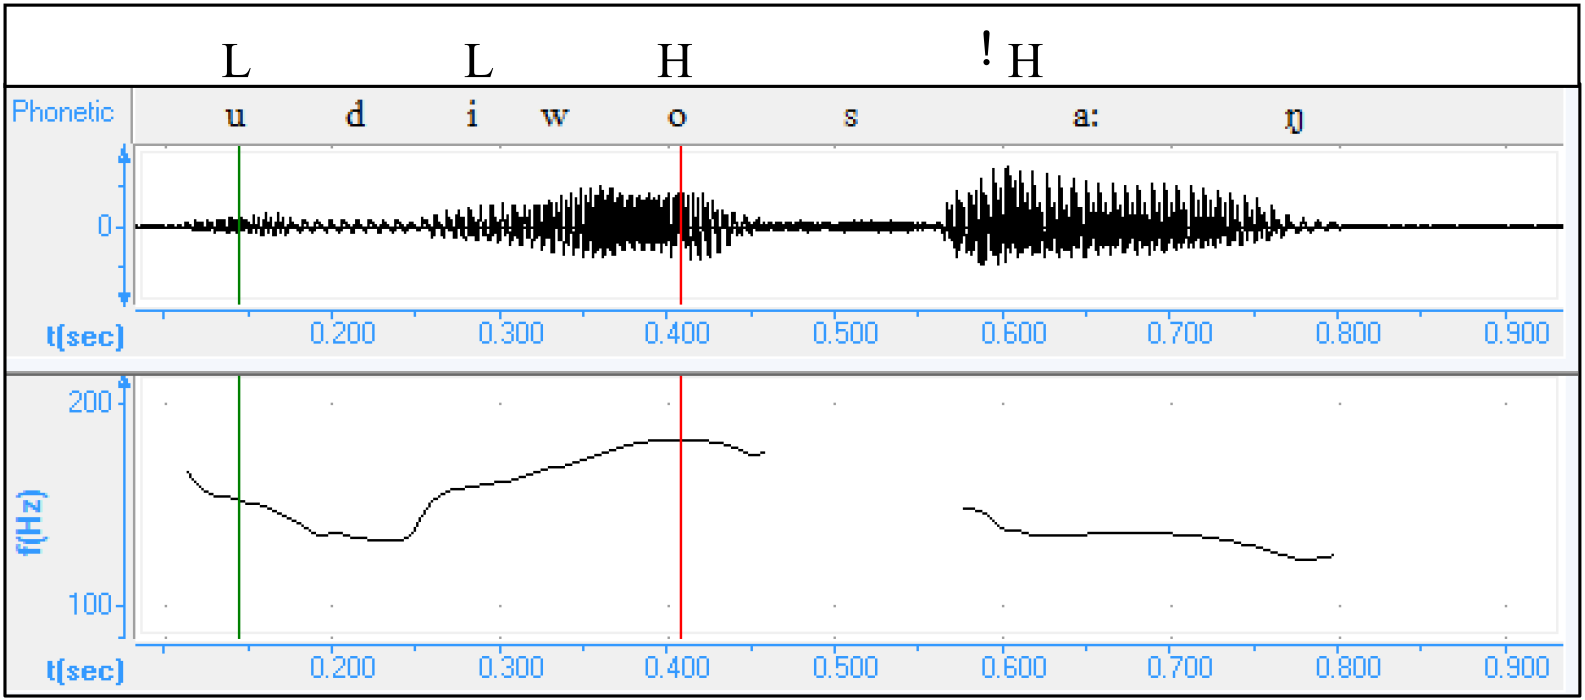
\includegraphics[width=\textwidth]{figures/cahillfig1}
\caption{\textit{\textbf{\underline{ù}} dìì-\textbf{\underline{wó}} \textit{\textsuperscript{!}}sááŋ}  `s/he ate TZ' (a type of porridge)}
\label{fig:1.cahill}
\end{figure}



The frequency, in Hertz \footnote{Reading the data in semitones is also an option in Speech Analyzer, and would be reported if there had been a mixed gender sample.} is read directly off a part of the graph not included in \figref{fig:1.cahill}. The frequency was read at either the stable part of the vowel or, lacking a flat portion of the frequency, at the midpoint of the vowel.  The \emph{base pitch level} in \figref{fig:1.cahill} is the frequency at the left cursor, i.e. at the Low toned [ù]. The \emph{pitch range} is the difference between this Low and the High of the [wó] syllable at the right cursor. 

Duration has also been found relevant in studies of other African languages \citep{hymanmonaka2011,fiedlerjannedy2013}, even when pitch is not directly involved. So the duration of the entire sentence was also measured, the distance between two cursors again being read directly off a part of the graph not included in \figref{fig:1.cahill}.

Regular and systematic differences were found between the neutral form of the utterance and the various emotional states for which data was gathered. We turn now to these. 

\section{Results} 
All the numbers reported in the following tables are averages of three utterances of that particular sentence. Frequencies are reported in Hertz (Hz), and duration is reported in milliseconds (ms). Other abbreviations in the tables are: 

\begin{itemize}
\item \EXP = expanded range (a larger L-H difference than the neutral)
\item \CONT = contracted range (a smaller L-H difference than the neutral)
\item ``l'' means that it's only slightly more of that quality, noticeable but with perhaps marginal significance 
\end{itemize}

As noted before, the requested \emph{surprise} intonation often elicited a polar question as the response. In terms of structural vs. paralinguistic intonation, the polar question exhibits both. As briefly mentioned above and detailed in \citet{cahill2012}, a polar question in Kɔnni is not only phonetically raised in pitch (paralinguistic), but is analyzable phonologically in terms of autosegments added to the neutral sentence (structural), and has one of several varieties of a falling tone on the final syllable. That syllable is categorically lengthened, and this accounts for the total duration of the \emph{surprise} intonation being lengthened in all the measurements to follow (thus the label ``longer'' rather than ``slower").



We begin with a detailed examination of results from one sentence, with separate charts for the two speakers. Each figure in the cells is the average from three repetitions. The columns L (Hz), H (Hz) and duration are all direct measurements, with the range (H-L) being derived from the first two. The last column sums up, in general terms, the difference between that emotional state and the neutral base form. 




\begin{table}
\resizebox{\textwidth}{!}{\begin{tabular}{llllll} 
\lsptoprule
& L (Hz) & H (Hz) & range (H-L) & duration & compared to neutral\\
\midrule
neutral & 128 & 153 & 25 & 798 & ---\\
bored & 128 & 157 & 29 & 810 & l-\EXP, l-slower\\
angry & 152 & 182 & 30 & 697 & higher, l-\EXP, faster\\
contemptuous & 147 & 177 & 30 & 738 & higher, l-\EXP, faster\\
emphatic & 135 & 172 & 37 & 743 & l-higher, \EXP, faster\\
surprise (no Q) & 156 & 185 & 29 & 703 & higher, l-\EXP, faster\\
\lspbottomrule
\end{tabular}}

\caption{`S/he has cooked yams' \emph{ù dìgìwó nyʊ́à} (Solomon)}
\label{tab:3.cahill}

\end{table}



\begin{table}
\resizebox{\textwidth}{!}{\begin{tabular}{llllll} 
\lsptoprule
& L (Hz) & H (Hz) & range (H-L) & duration & compared to neutral\\\midrule
neutral & 134 & 155 & 21 & 680 & ---\\
bored & 140 & 164 & 24 & 629 & l-higher, l-\EXP, faster\\
angry & 142 & 172 & 32 & 682 & higher, \EXP\\
contemptuous & 139 & 167 & 28 & 679 & l-higher, l-\EXP\\
emphatic & 142 & 180 & 38 & 706 & higher, \EXP, slower\\
surprise (ques) & 146 & 186 & 40 & 774 & higher, \EXP, longer\\
\lspbottomrule
\end{tabular}}

\caption{`S/he has cooked yams' \emph{ù dìgìwó nyʊ́à} (Salifu)}
\label{tab:4.cahill}

\end{table}



The first thing to note is that the two speakers had a few seemingly categorial differences in their expressions. Especially noteworthy is that the bored expression was slower than the neutral one for Solomon and faster for Salifu. Also, Solomon's angry and emphatic expressions were faster than Salifu's. There was other minor variation, but the main difference between speakers was speed in three utterances.

But more broadly, both speakers had results consistent with each other in that:

\begin{itemize}
\item bored was slightly expanded in range, a definite but not robust result
\item angry was definitely higher with an expanded range
\item contemptuous was slightly higher and slightly expanded, again definite but not robust
\item emphatic was higher, with an expanded range. 
\end{itemize}

On the surprise intonation, Salifu consistently responded by turning the statement into a polar (yes/no) question (`She has cooked yams?'). Solomon, however, uttered a non-question surprise intonation, which was higher and faster. It seems likely that pragmatically, the polar question is a more natural response to a surprising situation, but this cannot be verified at this point. 

Also, the pitch in a polar question in isolation is higher than in the corresponding statement, but the pitch in a polar question when someone is surprised is yet higher \citep{cahill2012}, and these two are quite distinguishable. The second situation is that which was produced and examined here.


Next we turn to a variety of input sentences, with the results of speaker Salifu. These are the same ones listed in \tabref{tab:2.cahill}.


\figref{fig:2.cahill} shows the aggregate results for pitch of the six sentences that Salifu repeated with neutral intonation and various emotional states. For this, the raw data measurements were used and combined. (Sentence-by sentence summary Tables are in the Appendix.) For each emotional state, the bottom measure is the initial Low tone of the sentence, and the second measure is the first High tone. Bars represent one standard deviation above and below the average.


\begin{figure}[h]
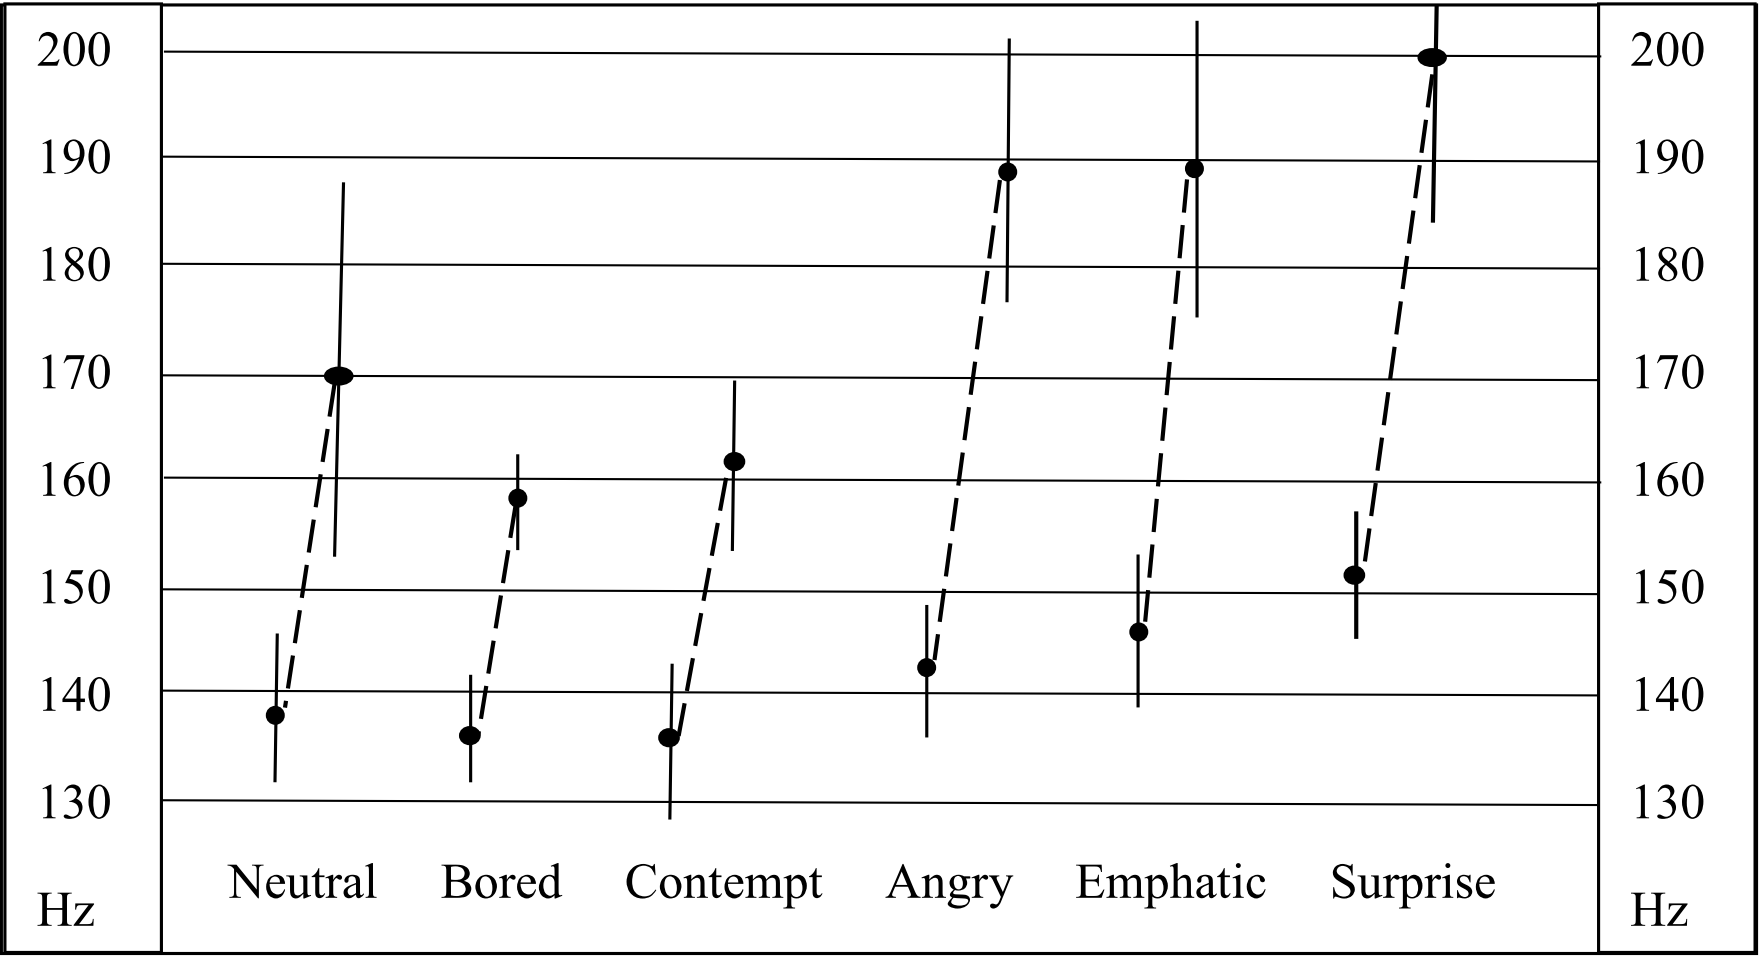
\includegraphics[width=\textwidth]{figures/cahillfig2}
\caption{Base pitch and first H tone -- a measure of height and of range}
\label{fig:2.cahill}
\end{figure}
 
As can be seen, the bored and contemptuous states have approximately the same starting pitch as neutral, but with the High of the sentences slightly lower than the neutral, they have a slightly narrower range.  The angry and emphatic states start slightly higher than neutral, but have a significantly larger pitch range.  The surprise intonation starts at the highest pitch of all (recall that Salifu turned this into a question), and also has a significantly larger pitch range than the neutral. At this point, as a rough approximation, the bored and contemptuous intonations appear quite similar to each other, as do the angry and emphatic, while surprise stands somewhat apart. 

Measurements of duration must be done sentence by sentence, since the target sentences are not uniform in syllable count. We would expect \textit{ʊ̀ chɔ̀gɪ̀sɪ̀wó \textsuperscript{!}bólíŋ}, with seven syllables, to have an inherently longer duration than the four syllables of \textit{ʊ̀ gàwá  \textsuperscript{!}nyʊ́ŋ}, and indeed in the neutral form they average 801 vs. 651 ms respectively. Thus the \emph{ratio} of the various emotive sentences to the neutral one is what is revealing, and these ratios are presented in \figref{fig:3.cahill}. 

\begin{figure}[h]
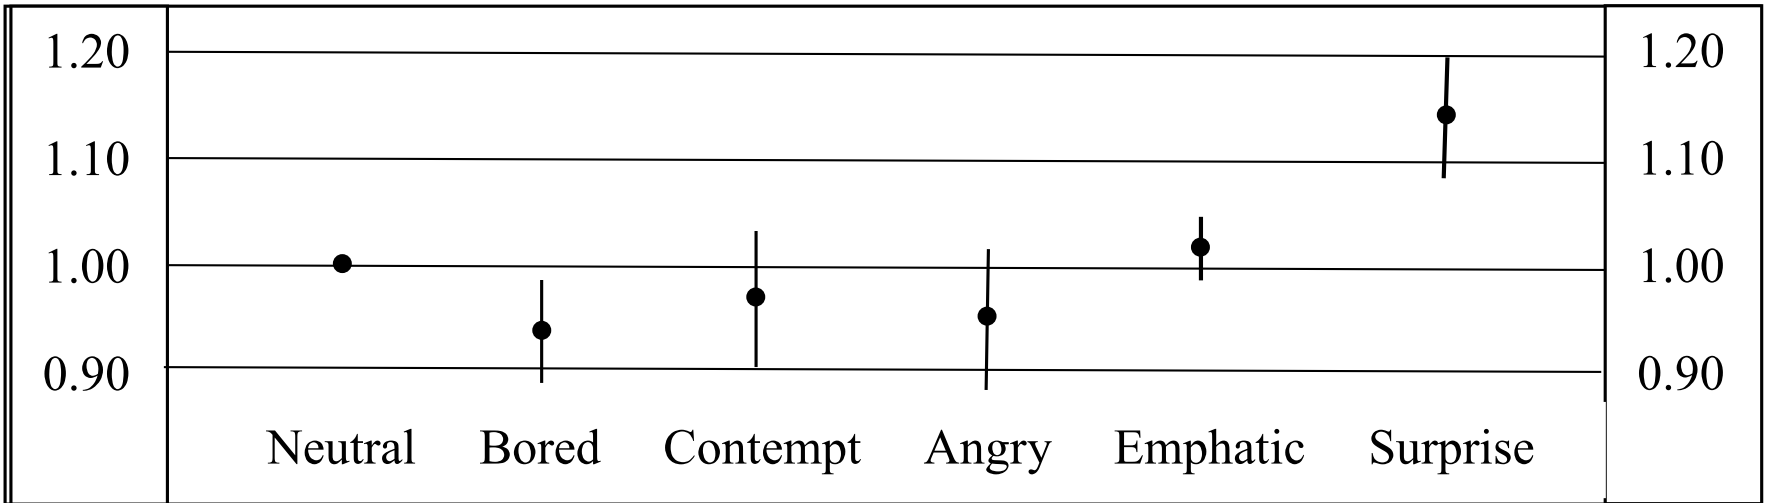
\includegraphics[width=\textwidth]{figures/cahillfig3}
\caption{Ratio of duration of emotive sentences to corresponding neutral sentence}
\label{fig:3.cahill}
\end{figure}

The duration of the surprise question is somewhat due to the extra mora added at the end of a polar question, as illustrated in \tabref{tab:1.cahill}. If 100 ms is subtracted from the average duration to account for this extra vowel, the duration of the surprise sentences drops closer to the range of the neutral. 

The duration of the emphatic sentence is worth singling out, as it contrasts with the other sentences (ignoring surprise for now) as being longer in duration than neutral. 

Several observations can be made on the basis of \figref{fig:2.cahill} and \figref{fig:3.cahill}. Again, actual data for these sentences is found in the Appendix.

\begin{itemize}
\item The bored expressions in Salifu's speech were consistently faster than the neutral ones, and most of the time had a contracted range. No consistent pattern of raising or lowering the base pitch was found.
\item The contemptuous expressions in Salifu's speech varied in speed, but were generally faster than neutral, and most of the time had a contracted range. Again, no consistent pattern of raising or lowering was found.
\item The bored and contemptuous patterns thus were quite similar to each other.
\item The angry expression was sometimes higher than neutral, mostly faster, but always with an expanded range.
\item The emphatic expression was always higher, always with expanded range, and almost always slower.
\item The surprise was always higher, with an expanded range, and longer. I use ``longer'' rather than ``slower'' because there is always an extra mora added.
\end{itemize}


\section{Summary and discussion}

A summary of generalizations is displayed in \tabref{tab:5.cahill}, with the caveat that these highest level generalizations conceal some detail. Besides previous measures, I also add some non-quantitative notes on volume/intensity , based on observations of the wave forms. 


\begin{table}
\begin{tabular}{lllll} 
\lsptoprule
& base pitch & range & speech rate & volume\\\midrule
bored & same & contracted & faster & quieter\\
contemptuous & same & contracted & varied/faster & quieter\\
angry & little higher & expanded & faster & same\\
emphatic & higher & expanded & slower & louder\\
surprise & higher & expanded & longer & louder\\
\lspbottomrule
\end{tabular}

\caption{Properties of emotions in Kɔnni, compared to neutral sentence intonation}
\label{tab:5.cahill}

\end{table}


Comparing the properties of the emotions in \tabref{tab:5.cahill} with Solomon's production of his one sentence and variants in \tabref{tab:3.cahill}, we see that the angry sentence had the same qualities for both speakers. The others were similar, but varied in one or more characteristics. As noted in the discussion after \tabref{tab:4.cahill}, the main speaker differences were in duration of the utterances.

The similarity between the bored and the contemptuous patterns may suggest that these are closely related in Kɔnni speakers' minds. It is easy to imagine that someone who is expressing contempt would act as if he were bored. However, other language studies have sometimes found overlap in pitch characteristics of unrelated emotions (see discussion of Thai in and around \tabref{tab:6.cahill} below), so phonetic likeness does not necessarily entail emotional similarity or identity. In light of the fact that there are different expressions for bored and contemptuous in Kɔnni (see discussion below), it seems more probable that these are merely phonetic overlaps of unrelated emotions.

If bored/contemptuous is counted as one intonation pattern, there are four distinct configurations of intonation that indicate emotional states in Kɔnni:

\begin{itemize}
\item A bored/contemptuous sentence is generally pronounced at a lower volume than neutral, with a contracted range, and faster than neutral. These all conspire together to reduce the overall prominence of the sentence.
\item An angry sentence is raised a bit, but its main characteristic is the expanded range and faster speed than neutral.
\item An emphatic sentence is significantly higher pitch than neutral, with expanded range, and a slower speed, the latter two of which presumably helps the hearer to clearly identify every word. The slower speed distinguishes this from the angry sentence.
\item A surprise sentence, even excluding the additional tonal and vocalic autosegments added to the final syllable, is also raised in pitch, with expanded range. It somewhat resembles the emphatic sentence in these respects. 
\end{itemize}

As noted in the title, this is must be regarded as quite a preliminary investigation; the results are suggestive and compatible with studies in other languages, but are too limited to be considered definitive. There are two obvious limitations to this study, one of which is more amenable to attack than the other. One limitation is limited data from a limited number of speakers, which could be remedied if time and conditions permitted. Secondly, and ideally, recordings would be made in natural settings rather than the artificial acting out that was done for this study. However, in such a situation, the amount of data collected in a reasonable amount of time would be a challenge, and control of the variables (the same sentence, number of repetitions, same speaker) would be very difficult. I know of no study which has actually put this into practice.

An obvious follow-up study is to see if other Kɔnni speakers can reliably identify the emotion acted out. It has been demonstrated that people can recognize the intonation patterns of some emotions, even cross-linguistically. \citet[72]{gussenhoven2004} cites \citet[128]{vanbezooijen1984} for a case of this. Taiwanese and Japanese speakers identified sadness, anger, and surprise by Dutch speakers at above chance levels. However, contempt and shame were not recognized. On the other hand, \citet[12]{garding1998} notes that Swedish emotional intonations are not so well established, and experiments have shown that Swedish speakers cannot distinguish happiness from anger by intonation alone. With the long-distance setup for this study, testing recognition of these emotional states by native Kɔnni speakers was impractical. Testing by speakers of other languages, particularly related African languages, would be a possible next step.

For an experiment of this type, where the aim is to collect data on intonation of different emotions from another language, a relevant question is if speakers of that language actually have that emotional category in their language, and words or expressions for it. Not all emotions translate directly, and if a speaker is aiming for an emotion that he or she is uncertain about, the results will also be uncertain and not dependable, both for that study and for comparative cross-linguistic purposes. In the midst of this writing, I inquired about this, and Konlan Kpeebi was able to confirm the following terms with another Kɔnni speaker, Mr. Ben Saibu, native Kɔnni speaker and lawyer. The terms for emotions in Kɔnni are the following.


\begin{enumerate}
\item Anger is straightforwardly termed \emph{sɩnyɩɩrɩŋ}.
\item Surprise is straightforwardly \emph{wuboŋkiŋ}. 
\item Boredom is expressed as \emph{wʋkpaaŋ} (the idea is ``too much talking/too many issues").
\item For contempt, there are actually several phrases: 

\begin{itemize}
\item \emph{dansɩ vuoŋ yɔɔrɩ} `look person nothing' (= he does not regard anyone) 
\item \emph{Ʋ nine ka suuli vuoŋ} `his eyes not fill person' (= he does not regard anyone) 
\item \emph{Ʋ ka daansɩ ye vuoŋ} `he does not look see person' (= he does not see anyone)
\end{itemize}
\item For emphasis, Saibu suggested \textit{Vii balɩ} which literally means `say it again', which would make the speaker assume the original hearer didn't quite understand it, and she or he should repeat it more understandably. This is not a direct translation of the English term \emph{emphasis}, but probably evokes the corresponding pronunciation.
\end{enumerate}

In general, then, it appears that Kɔnni does have reasonable lexical (and hence cultural) approximation for the emotional terms or categories elicited in this study. This also makes it more likely that the phonetic similarity between the bored and contemptuous intonations do not indicate that these emotions are identical in speakers' minds. 

The results of this study are compatible with those found in other languages, and specifically add to the knowledge of how tone languages are able to express paralinguistic intonation in a systematic way. For example, in German -- emphatic is ``more of everything", with a wider pitch range and longer duration \citep[91]{gibbon1998}.  In Swedish \citep[122--123]{garding1998}, anger has a wider pitch range. In Vietnamese (\citealt[402, 412--413]{doetal1998,brunelleetal2012}), anger has a comparatively shorter duration, greater pitch movement, increased loudness, and higher base pitch. Of the 13 attitudinal or emotive states for Thai reported in \citet[382]{luksaneeyanawin1998}, the ones that overlap with this study are presented in \tabref{tab:6.cahill}.\footnote{Pitch height being ``higher and lower'' in Luksaneeyanawin's terms means that pitch is higher for tones with a non-low starting point, and pitch is lower for the tones that have a low starting point. The ± symbol means that the quantity is sometimes enhanced, but not always.}


\begin{table}
\begin{tabular}{lllll}
\lsptoprule
 & pitch height & range & length & volume\\\midrule
bored & lower & narrower & shorter & softer\\
angry & higher \& lower & wider & ?? longer & very loud\\
emphatic & higher \& lower & wider & longer & louder\\
surprise & higher & narrower & ??shorter & ??louder\\
\lspbottomrule
\end{tabular}

\caption{Properties of emotions in Thai (extracted from \citealt[382]{luksaneeyanawin1998})}
\label{tab:6.cahill}

\end{table}



The 13 emotions have overlapping pitch characteristics in several cases, and \citeauthor{luksaneeyanawin1998} groups them into four \emph{tunes}. For example, the group with bored also has concealed anger in it, which may possibly have a connection to the contemptuous emotion in this study.

This study, preliminary and limited as it is, nonetheless illustrates definite patterns of how Kɔnni speakers vary their speech to express different emotional states. It also shows that the paralinguistic intonational variations that indicate states such as anger, emphasis, etc. have patterns that are similar to those documented for other languages, even tonal ones such as Thai. Whether these patterns are universal or merely common will depend on the results of more studies.


\section*{Appendix}

Each cell in these Tables reports the average of three repetitions.


\begin{table}
\caption{‘S/he went to market'	 \emph{ʊ̀ gàwá \textsuperscript{!}nyʊ́ŋ} (Salifu)}

\resizebox{\textwidth}{!}{\begin{tabular}{llllll} 
\lsptoprule
& L (Hz) & H (Hz) & range (H-L) & duration & compared to neutral\\\midrule
neutral & 150 & 189 & 39 & 651 & ---\\
bored & 135 & 169 & 34 & 552 & lower, l-\CONT, faster, quieter\\
angry & 150 & 203 & 53 & 558 & \EXP, faster, \~{} same intensity\\
contemptuous & 134 & 166 & 32 & 548 & lower, l-\CONT, faster, quieter\\
emphatic & 159 & 212 & 53 & 704 & higher, \EXP, slower, louder\\
surprise (Q) & 158 & 226 & 67 & 804 & higher, \EXP, longer\\
\lspbottomrule
\end{tabular}}
\end{table}

\begin{table}
\caption{‘S/he has bought oil'  \emph{ʊ̀ dààwá kpááŋ}  (Salifu)}

\resizebox{\textwidth}{!}{\begin{tabular}{llllll} 
\lsptoprule
& L (Hz) & H (Hz) & range (H-L) & duration & compared to neutral\\
\midrule
neutral & 134 & 144 & 10 & 700 & ---\\
bored & 140 & 155 & 15 & 629 & l-higher, l-\EXP, faster\\
angry & 140 & 172 & 32 & 682 & l-higher, \EXP, faster\\
contemptuous & 134 & 149 & 15 & 692 & l-\EXP, l-faster\\
emphatic & 145 & 172 & 27 & 717 & higher, \EXP, slower\\
surprise (Q) & 152 & 185 & 33 & 806 & higher, \EXP, longer\\
\lspbottomrule
\end{tabular}}
\end{table}

\begin{table}
 \caption{ ‘S/he has cooked eggs'  \emph{ù dìgìwó gɪ́là}  (Salifu)}

\resizebox{\textwidth}{!}{\begin{tabular}{llllll} \toprule
& L (Hz) & H (Hz) & range (H-L) & duration & compared to neutral\\\midrule
neutral & 139 & 162 & 23 & 658 & ---\\
bored & 139 & 158 & 19 & 614 & l-\CONT, faster\\
angry & 146 & 184 & 38 & 672 & l-higher, \EXP, slower\\
contemptuous & 144 & 165 & 21 & 669 & l-higher, l-\CONT, l-slower\\
emphatic & 146 & 181 & 35 & 668 & l-higher, \EXP, l-slower\\
surprise (Q) & 148 & 198 & 50 & 763 & higher, \EXP, longer\\
\lspbottomrule
\end{tabular}}
\end{table}

\begin{table}
\caption{‘S/he has fried eggs'   \emph{ʊ̀ chʊ̀ŋwá gɪ́là}  (Salifu)}

\resizebox{\textwidth}{!}{\begin{tabular}{llllll}
\lsptoprule
 & L (Hz) & H (Hz) & range (H-L) & duration & compared to neutral\\\midrule
neutral & 132 & 163 & 31 & 716 & ---\\
Bored & 133 & 156 & 23 & 683 & \CONT, faster\\
Angry & 130 & 181 & 51 & 716 & \EXP\\
contemptuous & 135 & 159 & 24 & 706 & \CONT, l-faster\\
emphatic & 142 & 184 & 42 & 725 & higher, \EXP, slower\\
surprise (Q) & 148 & 189 & 41 & 779 & higher, \EXP, longer\\
\lspbottomrule
\end{tabular}}
\end{table}

\begin{table}
\caption{‘S/he has eaten TZ'  \emph{ù dùùwó \textsuperscript{!}sááŋ}  (Salifu)}

\resizebox{\textwidth}{!}{\begin{tabular}{llllll} 
\lsptoprule
& L (Hz) & H (Hz) & range (H-L) & duration & compared to neutral\\\midrule
neutral & 139 & 173 & 34 & 697 & ---\\
bored & 137 & 162 & 25 & 679 & \CONT, faster\\
angry & \multicolumn{5}{l}{ Missing data}\\
contemptuous & 138 & 162 & 24 & 713 & \CONT, slower\\
emphatic & 143 & 191 & 48 & 713 & l-higher, \EXP, slower\\
surprise Q & 155 & 205 & 50 & 756 & higher, \EXP, longer\\
\lspbottomrule
\end{tabular}}
\end{table}

\begin{table}
\caption{‘S/he has fetched fire'  \emph{ʊ̀ chɔ̀gɪ̀sɪ̀wó \textsuperscript{!}bólíŋ}  (Salifu)}

\resizebox{\textwidth}{!}{\begin{tabular}{llllll}
\lsptoprule
& L (Hz) & H (Hz) & range (H-L) & duration & compared to neutral\\\midrule
neutral & 139 & 191 & 52 & 801 & ---\\
bored & 131 & 157 & 26 & 804 & lower, \CONT\\
angry & 136 & 200 & 64 & 760 & l-\EXP, faster\\
contemptuous & 132 & 169 & 37 & 779 & l-lower, \CONT, faster\\
emphatic & 142 & 199 & 57 & 802 & l-higher, l-\EXP\\
surprise Q & 148 & 196 & 48 & 909 & higher, \EXP, longer\\
\lspbottomrule
\end{tabular}}
\end{table}





\section*{Acknowledgements}
This study was first presented as a poster and handout at the 45th Annual Conference on African Linguistics at the University of Oregon in March 2014. I am grateful for discussions with various attendees there. Two anonymous referees and the editor, Doris Payne, made extremely valuable suggestions that have improved this paper immeasurably, and I thank them. Most of all, I thank Konlan and Solomon and Salifu for their crucial help in doing the recordings upon which this study was based.



\printbibliography[heading=subbibliography,notkeyword=this]


\end{document}